\documentclass[11pt]{scrartcl}
\usepackage[T1]{fontenc}
\usepackage[a4paper, left=3cm, right=2cm, top=2cm, bottom=2cm]{geometry}
\usepackage[activate]{pdfcprot}
\usepackage[ngerman]{babel}
\usepackage[parfill]{parskip}
\usepackage[utf8]{inputenc}
\usepackage[math]{kurier}
\usepackage{amsmath}
\usepackage{amssymb}
\usepackage{xcolor}
\usepackage{epstopdf}
\usepackage{txfonts}
\usepackage{fancyhdr}
\usepackage{graphicx}
\usepackage{prettyref}
\usepackage{hyperref}
\usepackage{eurosym}
\usepackage{setspace}
\usepackage{units}
\usepackage{eso-pic,graphicx}
\usepackage{icomma}
\usepackage{pdfpages}

\definecolor{darkblue}{rgb}{0,0,.5}
\hypersetup{pdftex=true, colorlinks=true, breaklinks=false, linkcolor=black, menucolor=black, urlcolor=darkblue}



\setlength{\columnsep}{2cm}


\newcommand{\arcsinh}{\mathrm{arcsinh}}
\newcommand{\asinh}{\mathrm{arcsinh}}
\newcommand{\ergebnis}{\textcolor{red}{\mathrm{Ergebnis}}}
\newcommand{\fehlt}{\textcolor{red}{Hier fehlen noch Inhalte.}}
\newcommand{\betanotice}{\textcolor{red}{Diese Aufgaben sind noch nicht in der Übung kontrolliert worden. Es sind lediglich meine Überlegungen und Lösungsansätze zu den Aufgaben. Es können Fehler enthalten sein!!! Das Dokument wird fortwährend aktualisiert und erst wenn das \textcolor{black}{beta} aus dem Dateinamen verschwindet ist es endgültig.}}
\newcommand{\half}{\frac{1}{2}}
\renewcommand{\d}{\, \mathrm d}
\newcommand{\punkte}{\textcolor{white}{xxxxx}}
\newcommand{\p}{\, \partial}
\newcommand{\dd}[1]{\item[#1] \hfill \\}

\renewcommand{\familydefault}{\sfdefault}
\renewcommand\thesection{}
\renewcommand\thesubsection{}
\renewcommand\thesubsubsection{}


\newcommand{\themodul}{Messtechnik}
\newcommand{\thetutor}{Prof. Helsper}
\newcommand{\theuebung}{Übungsklausur 2}

\pagestyle{fancy}
\fancyhead[L]{\footnotesize{C. Hansen}}
\chead{\thepage}
\rhead{}
\lfoot{}
\cfoot{}
\rfoot{}

\title{\themodul{}, \theuebung{}, \thetutor}


\author{Christoph Hansen \\ {\small \href{mailto:chris@university-material.de}{chris@university-material.de}} }

\date{}


\begin{document}

\maketitle

Dieser Text ist unter dieser \href{http://creativecommons.org/licenses/by-nc-sa/4.0/}{Creative Commons} Lizenz veröffentlicht.

\textcolor{red}{Ich erhebe keinen Anspruch auf Vollständigkeit oder Richtigkeit. Falls ihr Fehler findet oder etwas fehlt, dann meldet euch bitte über den Emailkontakt.}

\tableofcontents


\newpage



\section{Aufgabe 1}


Die richtigen Antworten sind:


\begin{center}
	\begin{tabular}{c|c|c|c|c|c|c|c}
				 1 & 2 & 3 & 4 & 5 & 6 & 7 & 8 \\ 
		\hline b,c & a & c & d & b,d & c & b & b,d \\  
	\end{tabular} 
\end{center}


\section{Aufgabe 2}

Wir haben eine Frequenz von $f = \frac{1}{\unit[4]{ms}} = \unit[250]{Hz}$

\subsection*{a)}

Die effektive Spannung können wir dann nach folgender Formel bestimmen:

\begin{align*}
U &= \sqrt{\frac{1}{T} \int_{0}^{T} U^2 \d t}
\intertext{Aus Symetriegründen reicht es hier über die halbe Periode zu integrieren:}
U(t) &= \unit[1]{V/ms} \cdot t \\
U^2 &= \frac{1}{2} \int_{0}^{\unit[2]{ms}} t^2 \d t = \frac{1}{2} \left[ \frac{1}{3} t^3 \right]_0^2  = \half \cdot \frac{1}{3} \cdot 8 = \unit[1,333]{V^2} \\
\hfill \\
\Rightarrow U &= \unit[1,155]{V}
\end{align*}

\subsection*{b)}

Das es eine reine Wechselgröße ist, zeigt das Messgerät $\unit[0]{V}$ an.


\subsection*{c)}


\paragraph{Schritt 1}

Wechselspannungseinkopplung

\paragraph{Schritt 2}

Gleichrichtung

\paragraph{Schritt 3}

arithmetischer Mittelwert

\begin{align*}
\bar{|U|} = \frac{1}{T} \int U \d t = \half \int_{0}^{2} 1 - t \d t = \left. \half t^2 \right|_0^2 = \unit[1]{V}
\end{align*}

\paragraph{Schritt 4}

Multiplikation mit Formfaktor für Sinus

\begin{align*}
U_\sim = 1,11111 \cdot 1 = \unit[1,1111]{V}
\end{align*}


\section{Aufgabe 3}

\subsection*{a)}


\begin{figure}[h]
	\centering
	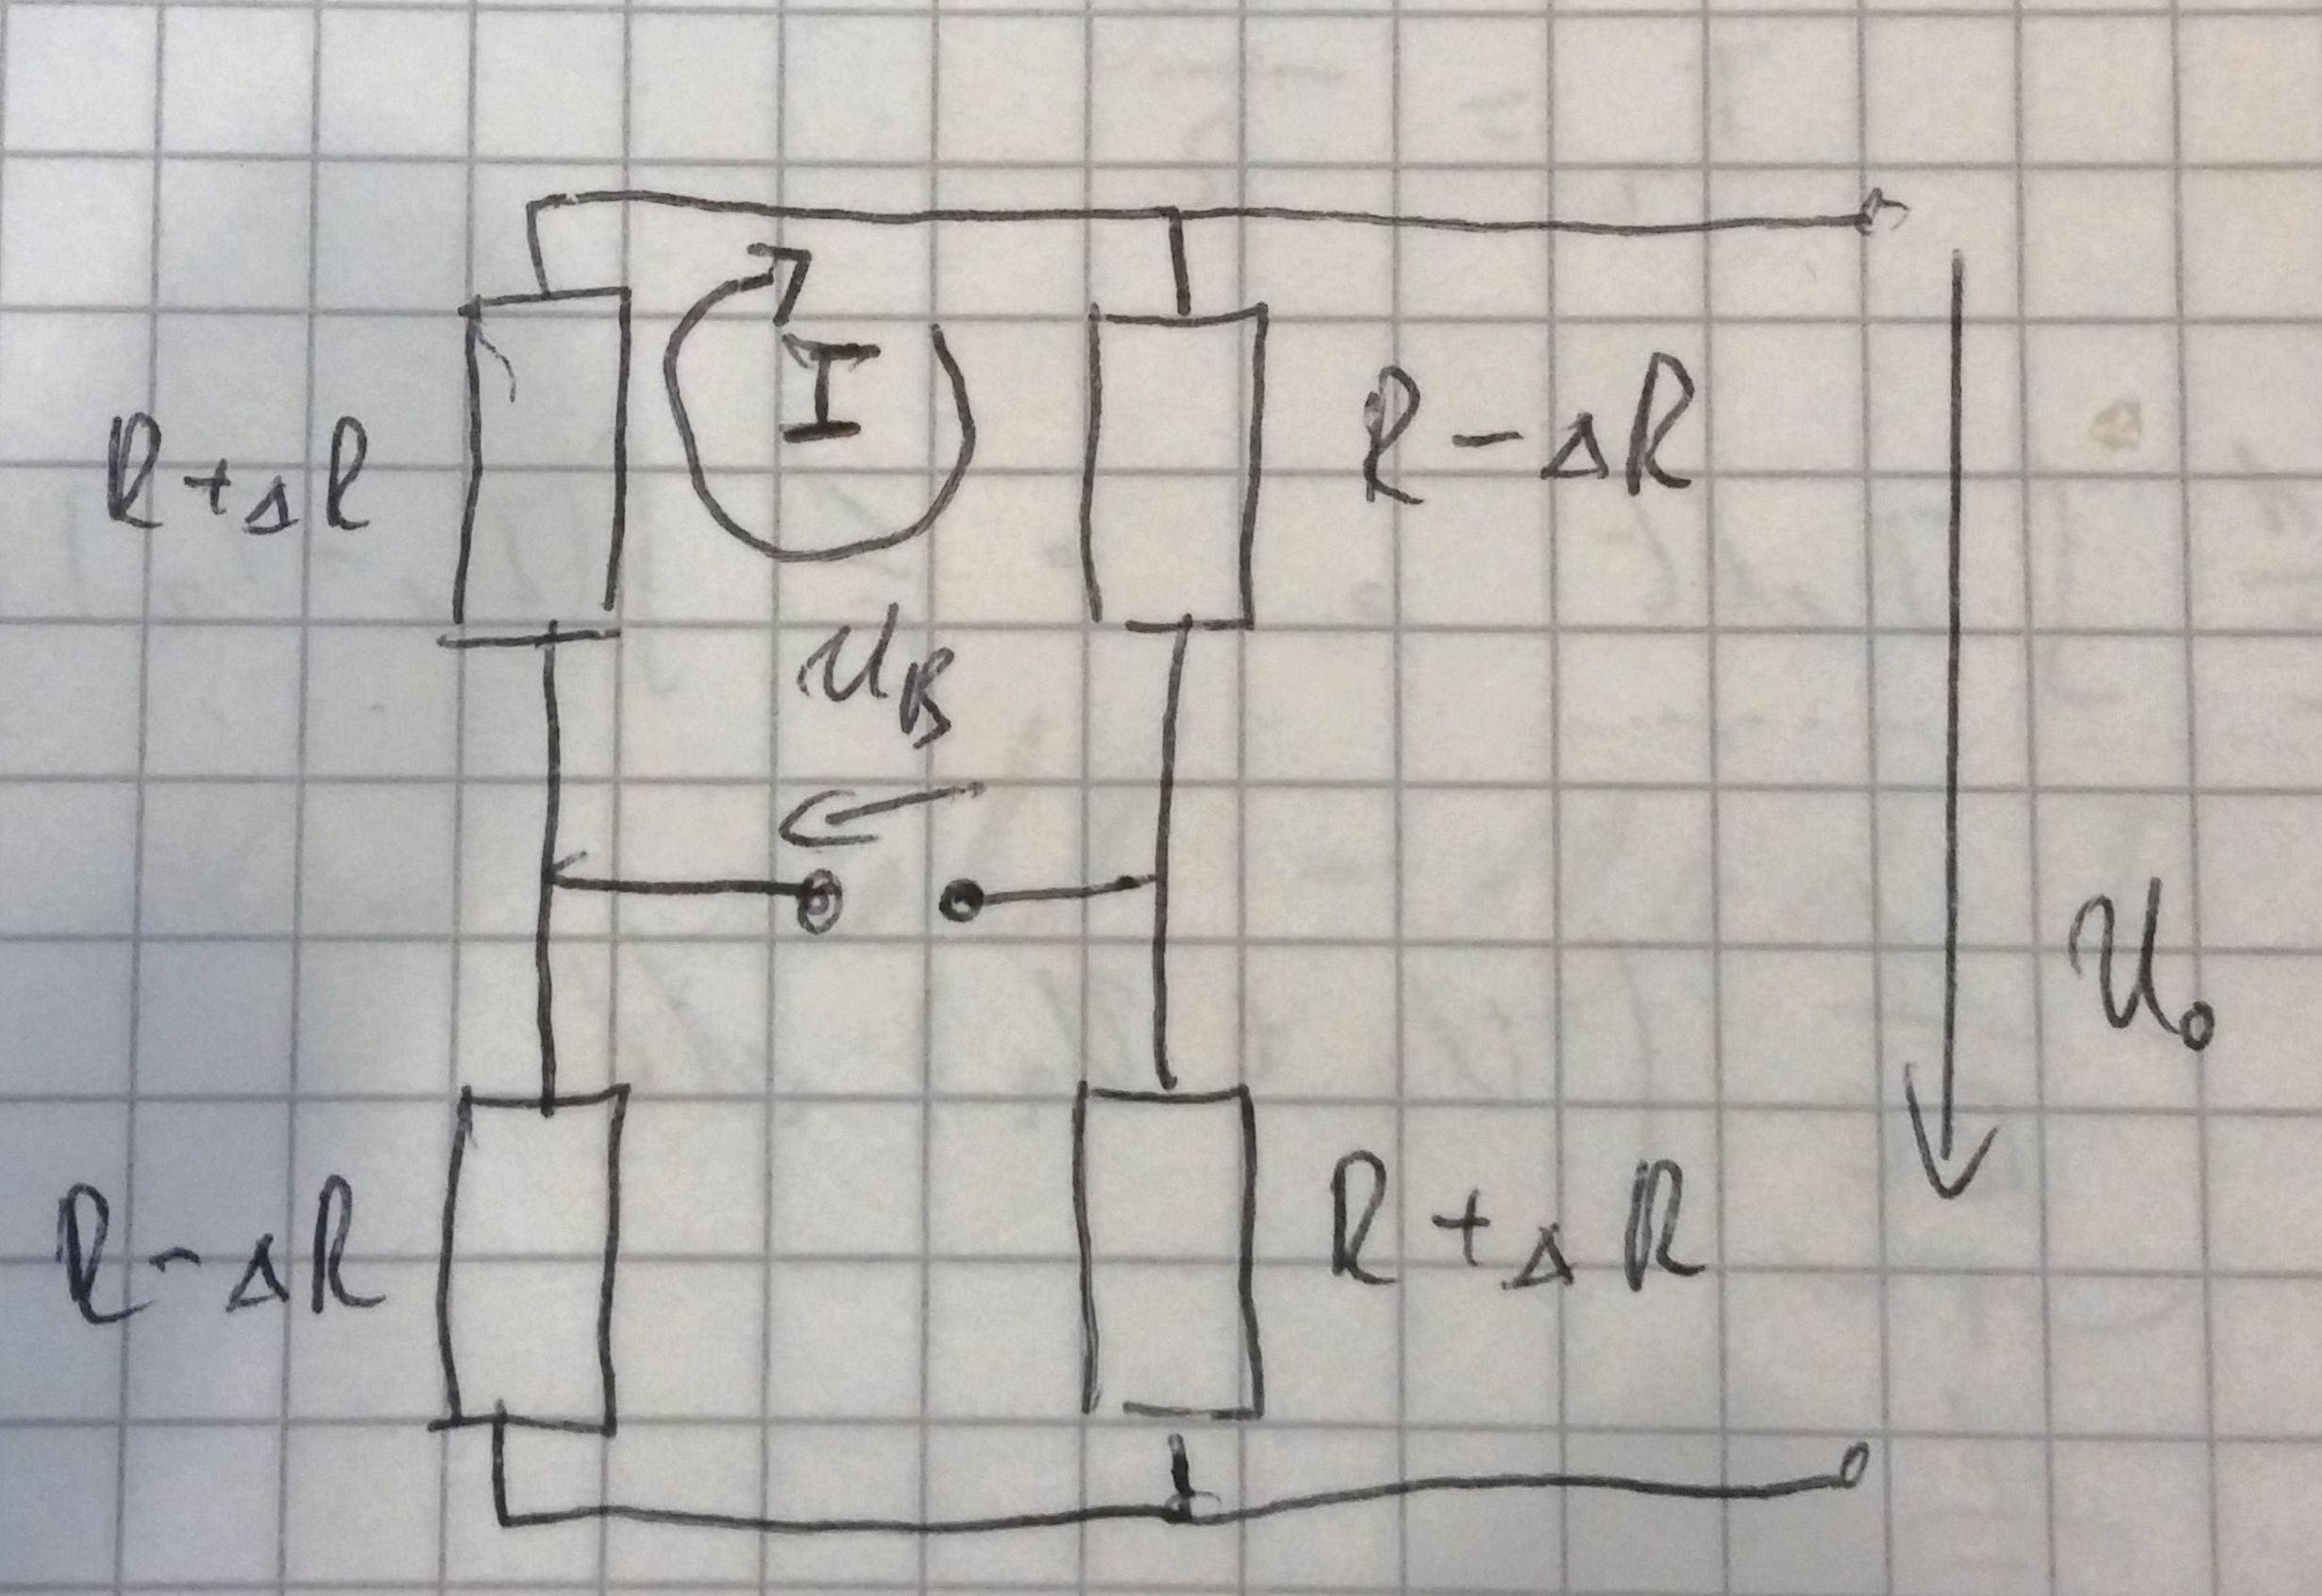
\includegraphics[scale=0.15]{A3_1.jpg}
\end{figure}


\subsection*{b)}

\begin{align*}
I_1 &= \frac{U_0}{R + \Delta R - \Delta R + R} = \frac{U_0}{2R} = I_2
\intertext{Wir betrachten nun die Masche I:}
0 &= I(R - \Delta R) + U_B - I(R + \Delta R) \\
\Leftrightarrow 0 &= \frac{U_0}{2R} \cdot R - \frac{U_0}{2R} \cdot \Delta R + U_B - \frac{U_0}{2R} \cdot R - \frac{U_0}{2R} \cdot \Delta R \\
\Leftrightarrow U_B &= \frac{\Delta R}{R} \cdot U_0
\end{align*}


\subsection*{c)}

\begin{align*}
\frac{\Delta R}{R} &= k \cdot \epsilon \\
\Leftrightarrow U_B &= k \cdot \epsilon \cdot U_O 
\intertext{Für die Empfindlichkeit müssen wir nach $\epsilon$ ableiten:}
E &= \frac{\p U_B}{\p \epsilon} = k \cdot U_0 = 2 \cdot 24 = \unit[48]{V}
\end{align*}


\section{Aufgabe 4}

\subsection*{a)}

Der Operationsverstärker ist invertierend , weil die Eingangsgröße auf $-$ liegt.

\subsection*{b)}

Es handelt sich um einen Integrierer (Kondensator) und Addierer (Anordnung der Eingangsspannungen)


\subsection*{c)}

\begin{align*}
I &= I_1 + I_2 \\
I_1 &= \frac{U_1}{R} \qquad I_2 = \frac{U_2}{R} \\
U_3 &= - \frac{1}{C} \int I \d t = - \frac{1}{C} \int I_1 + I_2 \d t \\
U_R &= \underbrace{ - \frac{1}{RC}}_{\frac{1}{T}} \int U_1 + U_2 \d t
\end{align*}

\subsection*{d)}

\begin{align*}
T &= RC \\ 
\Leftrightarrow C &= \frac{T}{e} = \frac{1}{100 \cdot 10^3} = \unit[10]{\mu F}
\end{align*}


\subsection*{e)}

Aufgabenteil fällt weg, weil outdated





\end{document}